\section{组合拉普拉斯}
\label{sec:graph-laplacian}

第~\ref{chap:graph-incidence-matrix}章的关联矩阵$\bm B$把顶点函数映射为沿边差分，又把边上的流量汇总到各顶点。如果将“沿边取差—乘以边权—按顶点汇总”三步复合起来，就得到顶点空间$\mathbb R^n$上的对称线性算子——组合拉普拉斯矩阵$\bm L$。本节依次介绍加权度与度矩阵、组合拉普拉斯矩阵的逐点定义以及它与关联矩阵的分解关系。

\subsection{加权度与度矩阵}
\label{sec:graph-weighted-adjacency}

沿用第~\ref{chap:graph-adjacency-matrix}章的记号。设有限无向无自环图$\mathcal G=(V,E)$有$n$个顶点、$m$条边，加权邻接矩阵$\bm W=(w_{i,j})\in\mathbb R^{n\times n}$在每对相邻顶点$(i,j)$处记录边权$w_{i,j}=w_{j,i}\geq 0$，无边处和对角线处均取零。

给定顶点函数$\bm x\in\mathbb R^n$，矩阵乘积$\bm W\bm x$的第$i$个分量把顶点$i$的所有邻居读数按对应边权加权求和：
\begin{equation}
  (\bm W\bm x)_i=\sum_{j=1}^n w_{i,j}\,x_j.
  \label{eq:graph-weighted-neighbor-sum}
\end{equation}
在图~\ref{fig:incidence-running-example}的四点五边单位权图上取读数$\bm x=(3,2,1,0)^\top$，第一行对顶点$1$的三个邻居$2,3,4$求和，得到$1\cdot2+1\cdot1+1\cdot0=3$；第二行只对顶点$2$的两个邻居$1$和$3$求和，得到$1\cdot3+1\cdot1=4$。如果把所有顶点的读数都取为常值$1$，顶点$1$的输出是$1+1+1=3$，而顶点$2$的输出是$1+1=2$。可见即使各点读数完全相同，$(\bm W\bm x)_i$的数值仍随顶点连接的总边权而不同。

将一个顶点的全部邻边权重相加，就得到该顶点的\term{加权度}（weighted degree），排成对角矩阵即得\emph{度矩阵}（degree matrix）：
\begin{equation}
  d_i=\sum_{j=1}^n w_{i,j}=(\bm W\bm 1)_i,\qquad
  \bm D=\operatorname{diag}(d_1,\ldots,d_n).
  \label{eq:graph-laplacian-weighted-degree}
\end{equation}
在单位权图中，$d_i$就是顶点$i$的邻居个数。若增大某条现有边的权重，只有该边两个端点的加权度随之增加，图的连接结构本身并不改变。由于所有边权非负，加权度$d_i=0$当且仅当顶点$i$关联的所有边权重全为零，即$i$是定义~\ref{def:positive-weight-support}中正权支撑$\mathcal G_+=(V,E_+)$的孤立顶点。

在四点五边算例中，顶点$1,3$各连接三个邻居，顶点$2,4$各连接两个邻居。当五条边均取单位权时，度向量为$\bm d=(3,2,3,2)^\top$；若仅把对角边$13$的权重改为$2$，则两端点$1$和$3$的加权度各增加$1$，度向量变为$(4,2,4,2)^\top$。除特别说明外，后文算例仍取全部边为单位权。

\subsection{组合拉普拉斯的定义}
\label{sec:graph-laplacian-matrix-form}

有了邻居加权和$\bm W\bm x$与度矩阵$\bm D$，就可以把“本点读数相对于各邻居读数的带权偏离总和”写成线性算子。对每条边$\{i,j\}$，用本点读数$x_i$减去邻居读数$x_j$，再乘上边权$w_{i,j}$；把顶点$i$所有邻边的带权差相加，就得到组合拉普拉斯在顶点$i$处的输出。

\begin{definition}[组合拉普拉斯矩阵]
\label{def:graph-combinatorial-laplacian}
设$\bm W$和$\bm D$分别为有限无向非负加权图的加权邻接矩阵和度矩阵。图的\term{组合拉普拉斯}（combinatorial Laplacian）矩阵$\bm L\in\mathbb R^{n\times n}$定义为
\begin{equation}
  (\bm L\bm x)_i=\sum_{j=1}^n w_{i,j}(x_i-x_j),\qquad
  \bm L=\bm D-\bm W.
  \label{eq:graph-combinatorial-laplacian}
\end{equation}
\end{definition}

将式~\eqref{eq:graph-combinatorial-laplacian}第一式按被减数与减数拆开：
\[
  (\bm L\bm x)_i
  =\sum_{j=1}^n w_{i,j}x_i - \sum_{j=1}^n w_{i,j}x_j
  =d_i x_i - (\bm W\bm x)_i.
\]
其中被减数部分$(\bm D\bm x)_i=d_i x_i$收集了本点读数的全部权重系数，减数部分$(\bm W\bm x)_i$则是式~\eqref{eq:graph-weighted-neighbor-sum}的邻居加权和，写成矩阵等式即为$\bm L=\bm D-\bm W$。

当$d_i>0$时，还可从邻域平均的角度理解这一输出。将$d_i$提取出来，式~\eqref{eq:graph-combinatorial-laplacian}可改写为
\[
  (\bm L\bm x)_i = d_i\left(x_i - \sum_{j=1}^n \frac{w_{i,j}}{d_i}x_j\right).
\]
括号内的求和是邻居读数按权重份额$w_{i,j}/d_i$（总和为$1$）计算的加权平均值，因此$(\bm L\bm x)_i$等于加权度$d_i$乘以本点读数高出邻居加权平均值的幅度。

定义~\ref{def:graph-combinatorial-laplacian}是按顶点逐行遍历邻居的写法；若改为按边逐条汇总，就能把$\bm L$与第~\ref{chap:graph-incidence-matrix}章的带符号关联矩阵$\bm B\in\mathbb R^{n\times m}$直接联系起来。固定每条边$e=\{i,j\}$的参考方向$i\to j$，关联矩阵的第$e$列为$\bm b_e=\bm e_i-\bm e_j$。将$\bm L$作用于顶点函数$\bm x$的过程可分解为先后衔接的三步：

第一步是沿边取差。左乘$\bm B^\top$将$n$维顶点函数$\bm x$映射为$m$维沿边差分向量$\bm B^\top\bm x$，其第$e$个分量为
\[
  (\bm B^\top\bm x)_e=\bm b_e^\top\bm x=x_i-x_j.
\]

第二步是按边乘权。左乘边权对角阵$\bm C=\operatorname{diag}(w_{e_1},\ldots,w_{e_m})$，将每条边的差值乘以该边的权重，得到带权边差向量$\bm C\bm B^\top\bm x$，其第$e$个分量为$w_e(x_i-x_j)$。

第三步是按顶点汇总。左乘$\bm B$把每条边的带权差送回它的两个端点：边$e$对应的单列项$w_e\bm b_e(\bm b_e^\top\bm x)$在尾端$i$处加上$w_e(x_i-x_j)$，在头端$j$处加上$-w_e(x_i-x_j)=w_e(x_j-x_i)$。将全部$m$条边的贡献叠加，即得组合拉普拉斯的关联矩阵分解：
\begin{equation}
  \bm L=\sum_{e\in E} w_e\bm b_e\bm b_e^\top
       =\bm B\bm C\bm B^\top.
  \label{eq:graph-laplacian-incidence-factorization}
\end{equation}

在式~\eqref{eq:graph-laplacian-incidence-factorization}的每一项秩一矩阵$w_e\bm b_e\bm b_e^\top$中，列向量$\bm b_e$出现两次。若反转边$e$的参考方向，$\bm b_e$变为$-\bm b_e$，两次负号相互抵消，故$\bm L$完全不依赖各边参考方向的选取。

图~\ref{fig:laplacian-readings-aggregation}在四点单位权图上展示了“沿边取差—乘边权—按顶点汇总”的三步过程。例如边$41$的参考方向为$4\to 1$，沿边差分为$x_4-x_1=0-3=-3$；汇总到头端顶点$1$时乘以$B_{1,41}=-1$得到$-(-3)=+3$，与边$12$送来的$+1$和边$13$送来的$+2$相加，给出$(\bm L\bm x)_1=6$。

\begin{BookInlineFigure}
  \centering
  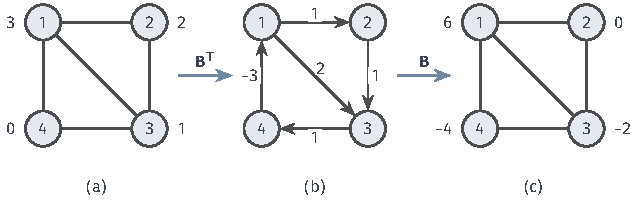
\includegraphics{figures/03-graphs/05-matrices-and-spectra/tikz/laplacian-readings-aggregation.pdf}
  \caption{四点单位权图上计算$\bm L\bm x$的三步分解。（a）顶点旁标注读数$\bm x=(3,2,1,0)^\top$。（b）箭头表示参考方向，边旁数字为沿边差分$\bm B^\top\bm x$（单位权下乘$\bm C$后不变）。（c）左乘$\bm B$汇总回各顶点的输出$\bm L\bm x=(6,0,-2,-4)^\top$。}
  \label{fig:laplacian-readings-aggregation}
\end{BookInlineFigure}

由分解式~\eqref{eq:graph-laplacian-incidence-factorization}立即可见：当所有顶点取同一常数$\bm x=c\bm 1$时，每条边两端读数相等，沿边差分$\bm B^\top(c\bm 1)=\bm 0$，从而$\bm L(c\bm 1)=\bm 0$。无论各顶点的加权度如何分布，全一常向量$\bm 1$始终属于$\bm L$的零空间。

在四点五边单位权算例中，将度向量$\bm d=(3,2,3,2)^\top$填入对角线，并在五条边对应的非对角位置各填$-1$，即得
\[
  \bm L=
  \begin{bmatrix}
  3&-1&-1&-1\\
  -1&2&-1&0\\
  -1&-1&3&-1\\
  -1&0&-1&2
  \end{bmatrix}.
\]
用单位脉冲$\bm e_1=(1,0,0,0)^\top$核对第一列：顶点$1$比三个邻居$2,3,4$各高出$1$，偏离总和为$3$；三个邻居$2,3,4$各自只有一个读数为$1$的邻居，偏离量均为$0-1=-1$，所得$(3,-1,-1,-1)^\top$恰好是$\bm L$的第一列。

\section{拉普拉斯二次型}
\label{sec:graph-laplacian-energy}

上一节给出了组合拉普拉斯矩阵$\bm L=\bm D-\bm W=\bm B\bm C\bm B^\top$及其对顶点函数$\bm x\in\mathbb R^n$的线性作用$\bm x\mapsto\bm L\bm x$。将线性输出$\bm L\bm x$与原向量$\bm x$作内积，就得到实对称矩阵$\bm L$所对应的二次型$\bm x^\top\bm L\bm x$。本节依次介绍拉普拉斯二次型的定义、半正定性等基本代数性质、它与图上顶点读数平滑性及子集割边权重的关系，最后简要介绍它在图分割与图信号处理中的应用。

\subsection{拉普拉斯二次型的定义}
\label{sec:graph-laplacian-quadratic-form}

在线性输出$(\bm L\bm x)_i=\sum_j w_{i,j}(x_i-x_j)$中，同一个顶点与不同邻居的一正一负差值会在求和时相互抵消。例如在三点单位权路径$1\!-\!2\!-\!3$上取$\bm x=(0,1,2)^\top$，中间顶点$2$与左邻$1$相差$+1$、与右邻$3$相差$-1$，相加得到$(\bm L\bm x)_2=0$，仅看该点输出看不出读数正在沿路径递增。

若改为考察二次型$\bm x^\top\bm L\bm x$，利用关联矩阵分解式~\eqref{eq:graph-laplacian-incidence-factorization}，可以把顶点空间上的内积$\bm x^\top(\bm L\bm x)$逐步转写到边空间上。记沿边差分向量为$\bm z=\bm B^\top\bm x\in\mathbb R^m$，其第$e$个分量（对应边$e=\{i,j\}$）为$z_e=x_i-x_j$，则
\[
  \begin{aligned}
    \bm x^\top\bm L\bm x
    &=\bm x^\top(\bm B\bm C\bm B^\top)\bm x\\
    &=(\bm B^\top\bm x)^\top\bm C(\bm B^\top\bm x)\\
    &=\bm z^\top\bm C\bm z\\
    &=\sum_{\{i,j\}\in E}w_{i,j}(x_i-x_j)^2.
  \end{aligned}
\]
若将关于无向边$\{i,j\}\in E$的求和改写为关于全体有序顶点对$(i,j)\in V\times V$的双重求和，每条无向边在$(i,j)$与$(j,i)$处各被计入一次，故须乘以因子$\frac12$。

\begin{definition}[拉普拉斯二次型与沿边变化能量]
\label{def:graph-dirichlet-energy}
设$\mathcal G=(V,E)$为有限无向非负加权图，$\bm L=\bm D-\bm W=\bm B\bm C\bm B^\top$为其组合拉普拉斯矩阵。对任意顶点函数$\bm x\in\mathbb R^n$，称
\begin{equation}
  \bm x^\top\bm L\bm x
  =\lVert\bm C^{1/2}\bm B^\top\bm x\rVert_2^2
  =\sum_{\{i,j\}\in E}w_{i,j}(x_i-x_j)^2
  =\frac12\sum_{i,j=1}^n w_{i,j}(x_i-x_j)^2
  \label{eq:graph-laplacian-energy}
\end{equation}
为$\bm x$的\emph{拉普拉斯二次型}（Laplacian quadratic form），也称为$\bm x$在图上的\term{沿边变化能量}（Dirichlet energy）。
\end{definition}

与逐点线性输出不同，式~\eqref{eq:graph-laplacian-energy}对每条边的两端差值$x_i-x_j$先平方再乘以边权$w_{i,j}$求和，因此不同边上的正负差值不再相互抵消。在刚才的三点路径上，$\bm x=(0,1,2)^\top$的二次型为$(0-1)^2+(1-2)^2=2$，真实反映了读数在两条边上的累积变化。

\subsection{拉普拉斯二次型的性质}
\label{sec:graph-laplacian-quadratic-properties}

由定义式~\eqref{eq:graph-laplacian-energy}中“加权平方和”的结构，可以直接导出组合拉普拉斯矩阵$\bm L$的半正定性以及二次型的平移不变性与边权可加性。

\begin{theorem}[拉普拉斯二次型的性质与半正定性]
\label{prop:graph-laplacian-quadratic-form}
设$\mathcal G=(V,E)$为有限无向非负加权图，组合拉普拉斯矩阵为$\bm L$。则：
\begin{enumerate}
  \item \emph{半正定性}：$\bm L$是实对称半正定矩阵，即对任意$\bm x\in\mathbb R^n$都有$\bm x^\top\bm L\bm x\geq 0$；且$\bm x^\top\bm L\bm x=0$当且仅当在每条正权边$\{i,j\}\in E_+$上都有$x_i=x_j$。
  \item \emph{常数平移不变性}：对任意$\bm x\in\mathbb R^n$和任意实数$c\in\mathbb R$，有
  \[
    (\bm x+c\bm 1)^\top\bm L(\bm x+c\bm 1)=\bm x^\top\bm L\bm x.
  \]
  \item \emph{关于边权的可加性与单调性}：若同一顶点集$V$上的两张非负加权图$\mathcal G_1,\mathcal G_2$按对应边权相加合成图$\mathcal G=\mathcal G_1+\mathcal G_2$，则对任意$\bm x\in\mathbb R^n$有
  \[
    \bm x^\top\bm L(\mathcal G)\bm x
    =\bm x^\top\bm L(\mathcal G_1)\bm x+\bm x^\top\bm L(\mathcal G_2)\bm x
    \geq\bm x^\top\bm L(\mathcal G_1)\bm x.
  \]
\end{enumerate}
\end{theorem}

\begin{proof}
（1）由$\bm W^\top=\bm W$和$\bm D^\top=\bm D$知$\bm L^\top=(\bm D-\bm W)^\top=\bm L$，故$\bm L$是实对称矩阵。在式~\eqref{eq:graph-laplacian-energy}中，由于每条边的权重$w_{i,j}\geq 0$且平方项$(x_i-x_j)^2\geq 0$，各项均非负，故$\bm x^\top\bm L\bm x\geq 0$，即$\bm L$半正定。非负项之和为零当且仅当每一项都为零；对于$w_{i,j}>0$的正权边$\{i,j\}\in E_+$，这等价于$(x_i-x_j)^2=0$，即$x_i=x_j$。

（2）将每个顶点的读数同时加上常数$c$后，任意一条边$\{i,j\}$两端的读数差为$(x_i+c)-(x_j+c)=x_i-x_j$，逐边差值完全不变，代入式~\eqref{eq:graph-laplacian-energy}即知二次型不变（这也与$\bm L\bm 1=\bm 0$一致）。

（3）当边权相加$w_{i,j}=w_{i,j}^{(1)}+w_{i,j}^{(2)}$时，由$\bm L=\sum_{e\in E}w_e\bm b_e\bm b_e^\top$对边权的线性性，有$\bm L(\mathcal G)=\bm L(\mathcal G_1)+\bm L(\mathcal G_2)$。左乘$\bm x^\top$、右乘$\bm x$即得二次型的可加性；再由$\bm x^\top\bm L(\mathcal G_2)\bm x\geq 0$立得不等式。
\end{proof}

\subsection{二次型与图结构}
\label{sec:graph-laplacian-cut-quadratic-form}

式~\eqref{eq:graph-laplacian-energy}将代数二次型$\bm x^\top\bm L\bm x$与图的拓扑连接紧密绑定在一起，主要体现在连续向量的沿边平滑度与离散子集的割边代价两个方面。

对于一般实向量$\bm x\in\mathbb R^n$，$\bm x^\top\bm L\bm x$度量了\emph{顶点函数沿图结构的平滑程度}。在求和式$\sum_{\{i,j\}\in E}w_{i,j}(x_i-x_j)^2$中，每一项都用边权$w_{i,j}$惩罚相邻顶点取值的不一致：如果图中相连的顶点（尤其是边权$w_{i,j}$较大的紧密连接顶点对）拥有相近的读数$x_i\approx x_j$，那么每条边上的$(x_i-x_j)^2$都很小，$\bm x^\top\bm L\bm x$就会非常小；反之，如果相邻顶点的读数剧烈反号或相差悬殊，$\bm x^\top\bm L\bm x$就会很大。

以四点五边单位权图为例，同样取长度为$2$的零和向量作比较。若取$\bm x=(1,1,-1,-1)^\top$，边$12$和边$34$两端读数相同（差为$0$），只有边$23,41,13$跨越正负号（差为$2$），二次型为$3\times 2^2=12$；若改为取$\bm x=(1,-1,1,-1)^\top$，四条外圈环边两端全部正负交替（差均为$2$），二次型增大为$4\times 2^2=16$。

当$\bm x=\bm 1_S$取为某个顶点子集$S\subseteq V$的$0$--$1$指示向量（在$i\in S$处取$1$，在$i\notin S$处取$0$）时，拉普拉斯二次型\emph{精确等于跨子集边界被切断的边的总权重（割边代价）}。对图中任意一条边$\{i,j\}\in E$，若两端点同在$S$内部或同在$V\setminus S$内部，则$\bm 1_S(i)=\bm 1_S(j)$，该边平方差为$0$；只有一端在$S$内、另一端在$V\setminus S$内的跨割边满足$|\bm 1_S(i)-\bm 1_S(j)|=1$，从而贡献其边权$w_{i,j}$：
\begin{equation}
  \bm 1_S^\top\bm L\bm 1_S
  =\sum_{\{i,j\}\in E}w_{i,j}(\bm 1_S(i)-\bm 1_S(j))^2
  =\sum_{i\in S,\,j\in V\setminus S}w_{i,j}
  =c(S,V\setminus S).
  \label{eq:graph-laplacian-cut-energy}
\end{equation}
同理，若用$\pm 1$指示向量$\bm s=2\bm 1_S-\bm 1$（在$S$内取$+1$，在$V\setminus S$内取$-1$）标记二分划分，则每条跨割边两端相差$2$、平方为$4$，从而$\bm s^\top\bm L\bm s=4\,c(S,V\setminus S)$。

图~\ref{fig:laplacian-edge-energy}在四点五边单位权图上展示了两个$0$--$1$指示向量的二次型。图~\ref{fig:laplacian-edge-energy}(a)取$S=\{1,3\}$的指示向量$\bm x=(1,0,1,0)^\top$，对角边$13$两端同在$S$内（差为$0$），四条外圈环边均跨越$S$与$\{2,4\}$（平方差各为$1$），故$\bm x^\top\bm L\bm x=4=c(\{1,3\},\{2,4\})$。图~\ref{fig:laplacian-edge-energy}(b)取单点集$S=\{1\}$的指示向量$\bm e_1=(1,0,0,0)^\top$，被切断的边恰好是与顶点$1$关联的三条边$12,41,13$，故$\bm e_1^\top\bm L\bm e_1=3=d_1$，这与对角元$L_{i,i}=\bm e_i^\top\bm L\bm e_i=d_i$完全一致。

\begin{BookInlineFigure}
  \centering
  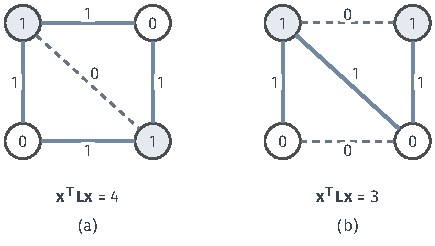
\includegraphics{figures/03-graphs/05-matrices-and-spectra/tikz/laplacian-edge-energy.pdf}
  \caption{四点单位权图上两个$0$--$1$指示向量的拉普拉斯二次型$\bm x^\top\bm L\bm x$。圆内为顶点读数，边旁为该边的平方差$(x_i-x_j)^2$。实线为跨割边（贡献$1$），虚线为同侧边（贡献$0$）。（a）$\bm x=\bm 1_{\{1,3\}}=(1,0,1,0)^\top$的二次型为$4$。（b）$\bm e_1=\bm 1_{\{1\}}=(1,0,0,0)^\top$的二次型为$3=d_1$。}
  \label{fig:laplacian-edge-energy}
\end{BookInlineFigure}

\subsection{在图问题中的应用}
\label{sec:graph-laplacian-quadratic-applications}

得益于“离散指示向量上等于割边代价、连续实向量上度量沿边平滑度”这一双重特性，拉普拉斯二次型在图算法与图数据分析中常作为核心目标函数或正则项出现。

第一类典型应用是\emph{图分割}（graph partitioning）。要把一张图切分为内部连接紧密、跨区连接稀疏的两个子集$S$与$V\setminus S$，就需要最小化跨子集的割边代价$c(S,V\setminus S)=\bm 1_S^\top\bm L\bm 1_S$，同时在子集大小$|S|$或连接体积上施加平衡约束，防止切出孤立小碎片。直接搜索最优离散子集是组合难问题；将离散指示向量松弛为满足正交与长度约束的连续实向量$\bm x\in\mathbb R^n$并最小化二次型$\bm x^\top\bm L\bm x$，离散割问题就转化为对称矩阵的瑞利商极值与特征向量计算问题，这也是第~\ref{chap:spectral-partition}章谱划分方法的出发点。

第二类典型应用是\emph{图信号处理中的去噪与平滑}（graph signal denoising and smoothing）。在传感器网络、社交网络或三维网格上，每个顶点带有一个观测读数$y_i$，排成观测向量$\bm y\in\mathbb R^n$。在采用图平滑先验的模型中，假设待恢复信号在相连顶点之间变化较小，而观测扰动会增加沿边差异；这一假设须与具体数据相符。将拉普拉斯二次型作为图平滑正则项加入最小二乘拟合，可构造如下去噪目标：
\begin{equation}
  \min_{\bm x\in\mathbb R^n}\Bigl\{\lVert\bm x-\bm y\rVert_2^2 + \gamma\,\bm x^\top\bm L\bm x\Bigr\}\qquad(\gamma>0),
  \label{eq:graph-laplacian-denoising}
\end{equation}
其中第一项要求恢复信号$\bm x$贴近观测$\bm y$，第二项以权重$\gamma$惩罚相连顶点之间的数值跳变。

由于$\bm L$半正定，式~\eqref{eq:graph-laplacian-denoising}的目标函数关于$\bm x$严格凸。对$\bm x$求梯度并令其为零，得到线性方程组
\[
  (\bm I+\gamma\bm L)\bm x=\bm y,\qquad
  \bm x=(\bm I+\gamma\bm L)^{-1}\bm y.
\]
该解在拟合观测与降低沿边变化之间作折中；若真实信号含有沿边突变，平滑正则化也可能引入偏差。类似地，若仅在部分边界顶点上已知标签读数，而在其余未知顶点上直接最小化沿边变化能量$\bm x^\top\bm L\bm x$，则得到图上的谐波插值与半监督标签传播；每个正权连通分量都含已知边界顶点时，未知读数唯一确定，其物理对应正是第~\ref{chap:graph-electrical-networks}章电网络中的最小能量原理。
